\chapter{Potensial Kimia dan Campuran}\label{ch:b2:chemical-potential}

Pada musim dingin, sebuah truk menaburkan garam di jalan yang tertutup es,
dan es itu mencair pada \qty{-10}{\celsius}; cairan pendingin mesin mobil,
air dengan sepertiga etana-1,2-diol, tidak membeku dalam embun beku malam
hari dan tidak mendidih di bawah kap mesin yang panas. Zat terlarut
menurunkan titik beku pelarutnya dan menaikkan titik didihnya, dan, untuk
larutan encer, besarnya bergantung pada jumlah partikel terlarut, bukan
pada jenisnya. Alat yang menjelaskannya adalah \omterm{def:b2:chemical-potential:chemical-potential}{potensial kimia}, yaitu
turunan parsial \omterm{def:b2:reaction-free-energy:gibbs-energy}{energi Gibbs} terhadap jumlah salah satu konstituen.
\omterm{def:b2:chemical-potential:chemical-potential}{Potensial kimia} menunjukkan ke mana setiap spesies ``ingin pergi'', di
antara fase-fase dan melalui reaksi, dan mengubah aktivitas, yang dalam
jilid Tahun 1 dipakai sebagai resep, menjadi besaran turunan.

\begin{recall}
\Cref{ch:b2:reaction-free-energy}: \omterm{def:b2:reaction-free-energy:gibbs-energy}{energi Gibbs} $G = H - TS$, $\dd G =
V\dd p - S\dd T + \Delta_r G\,\dd\xi$, kriteria evolusi $\Delta_r G\,
\dd\xi \leq 0$. Jilid Tahun 1 menuliskan aktivitas gas sebagai
$p_i/p^\circ$, aktivitas zat terlarut sebagai $c_i/c^\circ$, dan 1 untuk
padatan murni atau pelarut, serta mencatat bahwa dalam larutan ion pekat
aktivitas menyimpang dari konsentrasi, ``koreksi yang dibahas dalam jilid
Tahun 2''. Dari fisika: hukum gas sempurna, dan $(\partial G/\partial p)_T = V$
untuk zat murni.
\end{recall}

\begin{omfigure}

\includegraphics[width=0.58\linewidth]{images/book3/ai/b2-03-salt-spreader.jpg}

{\small Truk penabur garam menaburkan garam di jalan bersalju. Garam itu
larut dalam lapisan tipis air di atas es, dan larutannya membeku pada suhu
yang lebih rendah daripada air murni: es pun mencair.}
\end{omfigure}

\section{Besaran molar parsial}

Campurkan \qty{50}{mL} air dan \qty{50}{mL} etanol: volume campurannya
kurang dari \qty{100}{mL}. Dalam campuran, besaran ekstensif bukanlah
jumlah sumbangan zat-zat murninya; setiap konstituen menyumbang sesuai
dengan lingkungan sekitarnya.

\begin{definition}[Besaran molar parsial]\label{def:b2:chemical-potential:partial-molar}
Misalkan $X(T, p, n_1, \dots, n_k)$ adalah fungsi keadaan ekstensif sebuah
fase yang mengandung jumlah zat $n_1, \dots, n_k$. Yang disebut
\emph{besaran molar parsial}\index{besaran molar parsial} konstituen $i$
adalah
\[
  \bar X_i = \left(\frac{\partial X}{\partial n_i}\right)_{T, p, n_{j \ne i}} ,
\]
yaitu perubahan $X$ per mol $i$ yang ditambahkan ke sejumlah besar
campuran pada $T$, $p$, dan jumlah zat lain yang tetap. Untuk $X = V$,
besaran ini adalah \emph{volume molar parsial}\index{volume molar parsial}
$\bar V_i$.
\end{definition}

\begin{theorem}[Identitas Euler]\label{thm:b2:chemical-potential:euler}
Pada $T$ dan $p$ tetap, $X = \sum_i n_i\bar X_i$.
\end{theorem}

\begin{proof}
$X$ bersifat ekstensif: mengalikan setiap jumlah zat dengan $\lambda$
mengalikan $X$ dengan $\lambda$, $X(T, p, \lambda n_1, \dots, \lambda n_k) = \lambda X(T, p, n_1,
\dots, n_k)$. Turunkan terhadap $\lambda$ pada
$\lambda = 1$, dengan aturan rantai: $\sum_i n_i\,\partial X/\partial n_i = X$.
\end{proof}

\begin{proposition}[Hubungan Gibbs--Duhem]\label{prop:b2:chemical-potential:gibbs-duhem}
Pada $T$ dan $p$ tetap, $\sum_i n_i\,\dd\bar X_i = 0$: dalam campuran
biner, $x_1\dd\bar X_1 + x_2\dd\bar X_2 = 0$. Besaran-besaran molar parsial
para konstituen tidak dapat berubah secara bebas satu sama lain.
\end{proposition}

\begin{proof}
Pada $T$, $p$ tetap, $\dd X = \sum_i\bar X_i\dd n_i$ menurut definisi;
identitas Euler, jika diturunkan, memberikan $\dd X = \sum_i\bar X_i\dd n_i + \sum_i
n_i\dd\bar X_i$. Kurangkan keduanya.
\end{proof}

\begin{omfigure}
\begin{tikzpicture}
\begin{axis}[
  width=0.62\linewidth, height=5.4cm, xmin=0, xmax=1, ymin=8, ymax=62,
  axis x line=bottom, axis y line=left, xlabel={fraksi mol $x_2$},
  ylabel={volume molar $V_m$ (model)}, xtick={0,0.2,0.4,0.6,0.8,1}, ytick=\empty,
  tick label style={font=\small}, label style={font=\small}, ylabel shift=10pt, clip=false]
\addplot[omDef, very thick, domain=0:1, samples=60] {18*(1-x) + 58*x - 25*x*(1-x)};
\addplot[black!40, dashed, domain=0:1] {18*(1-x) + 58*x};
\addplot[omThm, thick, domain=0:1] {14 + 35*x};
\fill[omThm] (axis cs:0.4,28) circle (1.6pt);
\node[omThm, anchor=east, font=\small] at (axis cs:-0.01,14) {$\bar V_1$};
\node[omThm, anchor=west, font=\small] at (axis cs:1,49) {$\bar V_2$};
\node[font=\scriptsize, anchor=south east, black!60] at (axis cs:0.62,44) {jumlah volume murni};
\node[font=\small, anchor=north west] at (axis cs:0.41,27) {$x_2 = 0.4$};
\end{axis}
\end{tikzpicture}

{\small Konstruksi garis singgung. Volume molar sebuah campuran biner model
(biru) terletak di bawah garis lurus yang menghubungkan volume-volume
murninya: pencampuran menyebabkan penyusutan. Garis singgung pada suatu
komposisi memotong kedua tepi grafik pada \omterm{def:b2:chemical-potential:partial-molar}{volume molar parsial} $\bar V_1$
dan $\bar V_2$ untuk komposisi itu.}
\end{omfigure}

\begin{method}[Besaran molar parsial dari sebuah kurva]\label{met:b2:chemical-potential:tangent}
Alurkan besaran molar $X_m = X/(n_1 + n_2)$ terhadap $x_2$. Pada komposisi
yang dikehendaki, tariklah garis singgung: garis itu memotong sumbu
$x_2 = 0$ pada $\bar X_1$ dan sumbu $x_2 = 1$ pada $\bar X_2$. (Bukti:
$X_m = x_1\bar X_1 +
x_2\bar X_2$ dan, menurut Gibbs--Duhem,
$\dd X_m/\dd x_2 = \bar X_2 - \bar X_1$.)
\end{method}

\section{Potensial kimia}

\begin{definition}[Potensial kimia]\label{def:b2:chemical-potential:chemical-potential}
Yang disebut \emph{potensial kimia}\index{potensial kimia} konstituen $i$
dalam suatu fase adalah \omterm{def:b2:reaction-free-energy:gibbs-energy}{energi Gibbs} molar parsialnya,
\[
  \mu_i = \left(\frac{\partial G}{\partial n_i}\right)_{T, p, n_{j\ne i}} ,
\]
dalam \unit{J/mol}. Nilainya ketika $i$ berada dalam keadaan standarnya
adalah \emph{potensial kimia standar}\index{potensial kimia standar}
$\mu_i^\circ(T)$-nya, yang sama dengan \omterm{def:b2:reaction-free-energy:gibbs-energy}{energi Gibbs} molar standar $i$.
\end{definition}

Untuk fase yang jumlah zatnya dapat berubah (melalui reaksi, atau melalui
pertukaran dengan fase lain),
\[
  \dd G = V\dd p - S\dd T + \sum_i\mu_i\,\dd n_i ,\qquad G = \sum_i n_i\mu_i ,
\]
hubungan kedua berdasarkan identitas Euler. Dengan satu reaksi saja,
$\dd n_i =
\nu_i\dd\xi$, dan dengan membandingkannya dengan
\cref{prop:b2:reaction-free-energy:dG}:
\[
  \Delta_r G = \sum_i\nu_i\mu_i .
\]
\omterm{def:b2:reaction-free-energy:reaction-gibbs}{Energi Gibbs reaksi} adalah neraca \omterm{def:b2:chemical-potential:chemical-potential}{potensial kimia} produk dan \omterm{def:b2:chemical-potential:chemical-potential}{potensial
kimia} pereaksi.

\begin{theorem}[Kesetimbangan antarfase]\label{thm:b2:chemical-potential:phase-equilibrium}
Sebuah konstituen yang terdapat dalam dua fase $\alpha$ dan $\beta$ dari
sistem tertutup pada $T$ dan $p$ yang seragam berada dalam kesetimbangan
di antara kedua fase itu jika dan hanya jika $\mu_i^\alpha = \mu_i^\beta$.
Jika tidak, konstituen itu berpindah secara spontan dari fase tempat
\omterm{def:b2:chemical-potential:chemical-potential}{potensial kimianya} lebih tinggi ke fase tempat \omterm{def:b2:chemical-potential:chemical-potential}{potensial kimianya} lebih
rendah.
\end{theorem}

\begin{proof}
Perpindahan $i^\alpha \to i^\beta$ adalah sebuah ``reaksi'' dengan
$\nu^\alpha = -1$, $\nu^\beta = +1$, sehingga $\Delta_r G = \mu_i^\beta - \mu_i^\alpha$. Menurut kriteria evolusi, perpindahan itu maju
($\dd\xi > 0$) hanya jika $\mu_i^\beta <
\mu_i^\alpha$, mundur jika
$\mu_i^\beta > \mu_i^\alpha$, dan berada dalam kesetimbangan jika keduanya
sama.
\end{proof}

\omterm{def:b2:chemical-potential:chemical-potential}{Potensial kimia} memainkan peran bagi materi seperti peran suhu bagi kalor:
kalor mengalir dari yang panas ke yang dingin, sebuah spesies dari $\mu$
yang tinggi ke yang rendah.

\section{Sistem ideal dan aktivitas}

\begin{proposition}[Potensial kimia gas sempurna]\label{prop:b2:chemical-potential:mu-gas}
Dalam campuran gas sempurna, gas dengan tekanan parsial $p_i$ mempunyai
\[
  \mu_i = \mu_i^\circ(T) + RT\ln\frac{p_i}{p^\circ} .
\]
\end{proposition}

\begin{proof}
Untuk satu mol gas sempurna murni, $(\partial\mu/\partial p)_T = V_m =
RT/p$; integrasi dari $p^\circ$ sampai $p$ memberikan
$\mu = \mu^\circ + RT\ln(p/p^\circ)$. Dalam campuran gas sempurna, setiap
gas berperilaku seolah-olah sendirian di dalam volume itu, pada tekanan
parsialnya: gantilah $p$ dengan $p_i$.
\end{proof}

\begin{definition}[Campuran ideal, larutan encer ideal]\label{def:b2:chemical-potential:ideal-mixture}
Sebuah campuran cair (atau padat) disebut \emph{campuran
ideal}\index{campuran ideal} jika, untuk setiap konstituen dan setiap
komposisi, $\mu_i = \mu_i^*(T, p) + RT\ln x_i$, dengan $\mu_i^*$ \omterm{def:b2:chemical-potential:chemical-potential}{potensial
kimia} cairan murni $i$. Sebuah larutan disebut \emph{larutan encer
ideal}\index{larutan encer ideal} jika pelarutnya mematuhi hukum ini dan
setiap zat terlarut mematuhi $\mu_j = \mu_j^\circ(T) + RT\ln(c_j/c^\circ)$,
dengan keadaan standar berupa larutan hipotetis pada
$c^\circ = \qty{1}{mol/L}$ yang berperilaku seolah-olah sangat encer tak
berhingga.
\end{definition}

Molekul-molekul yang ukuran dan bentuknya serupa dan yang interaksinya
tidak bergantung pada pasangannya (benzena dan toluena, dua bentuk
isotopik sebuah molekul) membentuk campuran yang hampir ideal; larutan
encer berperilaku ideal karena setiap partikel zat terlarut hanya
dikelilingi oleh pelarut.

\begin{theorem}[Hukum Raoult]\label{thm:b2:chemical-potential:raoult}
Di atas campuran cair ideal, dengan uapnya berupa gas sempurna, tekanan
parsial setiap konstituen sebanding dengan fraksi molnya di dalam cairan:
$p_i = x_i\,p_i^*$, dengan $p_i^*$ tekanan uap cairan murni pada suhu yang
sama (\emph{hukum Raoult}\index{hukum Raoult}).
\end{theorem}

\begin{proof}
Pada kesetimbangan $\mu_i(\text{cair}) = \mu_i(\text{uap})$: $\mu_i^* +
RT\ln x_i = \mu_i^\circ + RT\ln(p_i/p^\circ)$. Untuk cairan murni
($x_i = 1$, $p_i = p_i^*$): $\mu_i^* = \mu_i^\circ + RT\ln(p_i^*/p^\circ)$.
Dengan mengurangkan keduanya, $RT\ln x_i = RT\ln(p_i/p_i^*)$.
(Kebergantungan $\mu_i^*$ yang lemah pada tekanan diabaikan.)
\end{proof}

\begin{proposition}[Hukum Henry]\label{prop:b2:chemical-potential:henry}
Untuk zat terlarut encer $j$ yang berada dalam kesetimbangan dengan
uapnya, $p_j = k_{H,j}\,x_j$ (atau $c_j = H_j\,p_j$): tekanan parsial zat
terlarut encer sebanding dengan jumlahnya di dalam larutan (\emph{hukum
Henry}\index{hukum Henry}). Yang disebut \emph{tetapan
Henry}\index{tetapan Henry} $k_{H,j}$ bergantung pada zat terlarut,
pelarut, dan suhu, dan bukan merupakan tekanan uap zat terlarut murni.
\end{proposition}

\begin{proof}
Samakan $\mu_j^\circ(\text{larutan}) + RT\ln(c_j/c^\circ)$ dan
$\mu_j^\circ(\text{gas}) + RT\ln(p_j/p^\circ)$: $c_j/p_j$ merupakan fungsi
$T$ saja. Tetapan itu memuat interaksi $j$ dengan pelarut, bukan dengan
dirinya sendiri.
\end{proof}

\begin{omfigure}
\begin{tikzpicture}
\begin{axis}[name=a,
  width=0.48\linewidth, height=5.6cm, xmin=0, xmax=1, ymin=0, ymax=1.5,
  axis x line=bottom, axis y line=left, xlabel={$x_1$}, ylabel={$p/p_1^*$},
  xtick={0,0.5,1}, ytick={0,0.5,1,1.5},
  tick label style={font=\small}, label style={font=\small}, title={\small ideal}]
\addplot[omDef, thick] table[x=x1, y=p1] {figdata/out/bachelor-2-raoult-henry-ideal.dat};
\addplot[omThm, thick] table[x=x1, y=p2] {figdata/out/bachelor-2-raoult-henry-ideal.dat};
\addplot[black, very thick] table[x=x1, y=p] {figdata/out/bachelor-2-raoult-henry-ideal.dat};
\node[omDef, font=\scriptsize, anchor=west] at (axis cs:0.55,0.42) {$p_1$};
\node[omThm, font=\scriptsize, anchor=west] at (axis cs:0.1,0.42) {$p_2$};
\node[font=\scriptsize, anchor=south] at (axis cs:0.5,0.8) {$p$};
\end{axis}
\begin{axis}[at={(a.east)}, anchor=west, xshift=1.2cm,
  width=0.48\linewidth, height=5.6cm, xmin=0, xmax=1, ymin=0, ymax=1.5,
  axis x line=bottom, axis y line=left, xlabel={$x_1$},
  xtick={0,0.5,1}, ytick={0,0.5,1,1.5},
  tick label style={font=\small}, label style={font=\small}, title={\small simpangan positif}]
\addplot[omDef, thick] table[x=x1, y=p1] {figdata/out/bachelor-2-raoult-henry-margules.dat};
\addplot[omThm, thick] table[x=x1, y=p2] {figdata/out/bachelor-2-raoult-henry-margules.dat};
\addplot[black, very thick] table[x=x1, y=p] {figdata/out/bachelor-2-raoult-henry-margules.dat};
\addplot[omDef, densely dashed, domain=0.6:1] {x};
\addplot[omDef, dotted, thick, domain=0:0.42] {3.004166*x};
\node[omDef, font=\scriptsize, anchor=west] at (axis cs:0.62,0.5) {Raoult};
\node[omDef, font=\scriptsize, anchor=east] at (axis cs:0.27,1.18) {Henry};
\node[omDef, font=\scriptsize, anchor=north west] at (axis cs:0.8,0.78) {$p_1$};
\node[omThm, font=\scriptsize, anchor=north] at (axis cs:0.55,0.24) {$p_2$};
\node[font=\scriptsize, anchor=south] at (axis cs:0.5,1.23) {$p$};
\end{axis}
\end{tikzpicture}

{\small Tekanan uap di atas cairan biner pada suhu tetap, dalam satuan
$p_1^*$ (campuran model). Kiri, \omterm{def:b2:chemical-potential:ideal-mixture}{campuran ideal}: garis-garis lurus
(Raoult). Kanan, campuran yang molekul-molekul tak sejenisnya saling
menarik lebih lemah daripada molekul-molekul sejenis: tekanannya terletak
di atas garis ideal. Di dekat $x_1 = 1$, konstituen 1 mengikuti garis
Raoult (putus-putus); di dekat $x_1 = 0$, konstituen itu mengikuti garis
Henry (titik-titik) dengan kemiringan yang berbeda.}
% (computed in figdata/bachelor-2/raoult-henry.py; Margules parameter 1.1, model)
\end{omfigure}

\begin{example}[Karbon dioksida dalam minuman soda]\label{ex:b2:chemical-potential:soda}
Pada \qty{25}{\celsius}, \omterm{prop:b2:chemical-potential:henry}{tetapan Henry} karbon dioksida dalam air adalah
$H =
\qty{3.4e-4}{mol/(m^3.Pa)}$, yaitu \qty{0.034}{mol/(L.bar)}. Botol
yang ditutup di bawah \qty{4}{bar} \ce{CO2} mengandung $0.034 \times 4 =
\qty{0.14}{mol/L}$ gas terlarut, sekitar \qty{6}{g/L}. Setelah dibuka, gas
di atasnya adalah udara, dengan $p_{\ce{CO2}} \approx \qty{4e-4}{bar}$:
minuman itu sepuluh ribu kali lewat jenuh dan terus berbuih sampai
gasnya habis.
% ledger: henry:CO2, air:CO2
\end{example}

\begin{proposition}[Aktivitas dari potensial kimia]\label{prop:b2:chemical-potential:activity}
Dalam semua kasus yang sejauh ini dijumpai, $\mu_i = \mu_i^\circ(T) + RT\ln a_i$, dengan $a_i$ aktivitas dari jilid Tahun 1: $p_i/p^\circ$ untuk
gas sempurna, $c_i/c^\circ$ untuk zat terlarut dalam \omterm{def:b2:chemical-potential:ideal-mixture}{larutan encer ideal},
$x_i$ (mendekati 1) untuk pelarut, dan 1 untuk padatan atau cairan murni
yang sendirian dalam fasenya.
\end{proposition}

\begin{proof}
Untuk gas dan zat terlarut encer, inilah isi
\cref{prop:b2:chemical-potential:mu-gas} dan definisi \omterm{def:b2:chemical-potential:ideal-mixture}{larutan encer
ideal}. Untuk konstituen \omterm{def:b2:chemical-potential:ideal-mixture}{campuran ideal}, ambillah cairan murni sebagai
keadaan standarnya: $a_i = x_i$, mendekati 1 untuk pelarut. Padatan atau
cairan murni adalah keadaan standarnya sendiri (kebergantungannya yang
lemah pada tekanan diabaikan): $\mu = \mu^\circ$, $a = 1$.
\end{proof}

\begin{proposition}[Energi Gibbs reaksi dan kuosien reaksi]\label{prop:b2:chemical-potential:delta-g-q}
Untuk reaksi $0 = \sum_i\nu_i\mathrm A_i$,
\[
  \Delta_r G = \Delta_r G^\circ(T) + RT\ln Q, \qquad Q = \prod_i a_i^{\nu_i} .
\]
\end{proposition}

\begin{proof}
$\Delta_r G = \sum_i\nu_i\mu_i = \sum_i\nu_i\mu_i^\circ + RT\sum_i\nu_i\ln a_i =
\Delta_r G^\circ + RT\ln\prod_i a_i^{\nu_i}$.
\end{proof}

Inilah jembatan antara \omterm{def:b2:reaction-free-energy:gibbs-energy}{energi Gibbs} pada \cref{ch:b2:reaction-free-energy}
dan kuosien reaksi dari jilid Tahun 1. Bab berikutnya menyeberanginya.

\begin{method}[Memilih keadaan acuan sebuah aktivitas]\label{met:b2:chemical-potential:activity-reference}
\begin{enumerate}
  \item Gas: gas sempurna murni pada $p^\circ$; $a = p_i/p^\circ$.
  \item Pelarut, atau konstituen campuran dengan jumlah yang sebanding:
        cairan murni; $a = \gamma_i x_i$ (acuan Raoult, $\gamma_i \to 1$
        ketika $x_i \to 1$).
  \item Zat terlarut: larutan ideal pada $c^\circ$; $a = \gamma_j c_j/c^\circ$
        (acuan Henry, $\gamma_j \to 1$ pada pengenceran tak berhingga).
  \item Padatan murni, cairan murni yang sendirian dalam fasenya: $a = 1$.
\end{enumerate}
\end{method}

\begin{history}[François-Marie Raoult]
\begin{minipage}[t]{0.2\linewidth}\vspace{0pt}
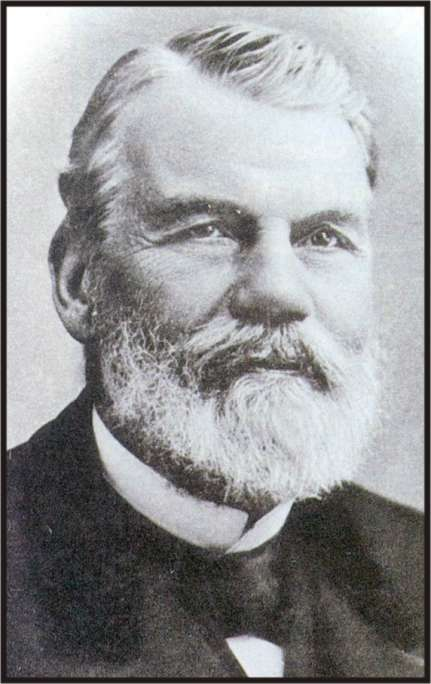
\includegraphics[width=\linewidth]{images/book3/raoult.jpg}
\end{minipage}\hfill
\begin{minipage}[t]{0.76\linewidth}\vspace{0pt}
François-Marie Raoult (1830--1901), profesor kimia di Grenoble, pada
tahun 1880-an mengukur titik beku dan kemudian tekanan uap ratusan
larutan, dan mendapati bahwa, untuk larutan encer, penurunannya
bergantung pada jumlah molekul terlarut, bukan pada jenisnya. Hasil
pengukurannya menjadi cara untuk ``menimbang'' molekul, dan mendukung
teori ion dalam larutan yang waktu itu masih muda. (Foto: domain publik,
Wikimedia Commons.)
\end{minipage}
\end{history}

\section{Campuran nyata}

\begin{definition}[Koefisien aktivitas]\label{def:b2:chemical-potential:activity-coefficient}
Dalam campuran nyata, \omterm{def:b2:chemical-potential:chemical-potential}{potensial kimia} dituliskan $\mu_i = \mu_i^\circ +
RT\ln a_i$ dengan $a_i = \gamma_i x_i$ (acuan Raoult) atau $a_i = \gamma_i
c_i/c^\circ$ (acuan Henry). Faktor $\gamma_i$ disebut \emph{koefisien
aktivitas}\index{koefisien aktivitas}: faktor ini mengukur penyimpangan
dari hukum ideal, dan menuju 1 dalam limit tempat hukum acuan itu berlaku.
\end{definition}

Koefisien di atas 1 berarti bahwa molekul itu kurang distabilkan oleh
tetangga-tetangganya di dalam campuran dibandingkan dalam keadaan acuan
(simpangan positif, seperti pada gambar di atas); di bawah 1, lebih
distabilkan. Menurut Gibbs--Duhem, koefisien kedua konstituen campuran
biner saling terkait: dalam model satu parameter yang dipakai untuk gambar
itu, $\ln\gamma_1 = Ax_2^2$ dan $\ln\gamma_2 = Ax_1^2$, dan
$x_1\,\dd\ln\gamma_1 + x_2\,\dd\ln\gamma_2 = 0$ berlaku secara identik.

Untuk ion, yang berinteraksi pada jarak jauh, penyimpangan sudah muncul
pada konsentrasi kecil.

\begin{definition}[Kekuatan ion]\label{def:b2:chemical-potential:ionic-strength}
Yang disebut \emph{kekuatan ion}\index{kekuatan ion} sebuah larutan adalah
$I =
\frac12\sum_i z_i^2\,b_i$, dengan $b_i$ molalitas ion $i$ (jumlah zat
per kilogram pelarut) dan $z_i$ bilangan muatannya.
\end{definition}

\begin{proposition}[Hukum pembatas Debye--Hückel]\label{prop:b2:chemical-potential:debye-huckel}
Dalam larutan elektrolit yang sangat encer, \omterm{def:b2:chemical-potential:activity-coefficient}{koefisien aktivitas} rata-rata
ion-ion sebuah garam mematuhi
$\log\gamma_\pm = -A\,|z_+z_-|\sqrt{I/b^\circ}$, dengan $A
\approx 0.51$
untuk air pada \qty{25}{\celsius} dan $b^\circ =
\qty{1}{mol/kg}$.
\end{proposition}
\admitted

\begin{remark}[Daerah berlaku dan asal-usulnya]\label{rem:b2:chemical-potential:dh-range}
Hukum ini berasal dari model yang menganggap setiap ion dikelilingi oleh
``atmosfer'' difus bermuatan berlawanan, yang menurunkan \omterm{def:b2:chemical-potential:chemical-potential}{potensial
kimianya}; model itu berada di luar cakupan kuliah ini, tetapi tetapan $A$
diperoleh dari permitivitas dan massa jenis air serta suhu. Hukum ini
akurat di bawah sekitar $I = \qty{0.01}{mol/kg}$. Atmosfer ion yang sama
memperlambat ion-ion dalam medan listrik, dan menjelaskan mengapa
konduktivitas molar elektrolit kuat menurun menurut
$\Lambda = \Lambda^\circ - K\sqrt c$ (hukum akar kuadrat Kohlrausch)
alih-alih tetap pada nilai batasnya: inilah batas hukum Kohlrausch yang
dijumpai dalam jilid Tahun 1.
% ledger: epsr:H2O, rho:water.298, const:e, const:eps0, const:kB, const:NA (A computed in figdata/bachelor-2/colligative.py)
\end{remark}

\begin{example}[Garam sentimolar]\label{ex:b2:chemical-potential:dh}
Untuk natrium klorida pada $b = \qty{0.010}{mol/kg}$, $I = \frac12(0.010 + 0.010)
= \qty{0.010}{mol/kg}$ dan $\log\gamma_\pm = -0.51 \times 0.10$:
$\gamma_\pm
= 0.89$. Pada seperseratus mol per kilogram saja, menganggap
konsentrasi sebagai aktivitas sudah merupakan galat 11\,\%; untuk garam 2:2
seperti magnesium sulfat pada molalitas yang sama, $I = 0.040$ dan
$\gamma_\pm = 0.62$.
\end{example}

\section{Sifat koligatif}

\begin{definition}[Sifat koligatif]\label{def:b2:chemical-potential:colligative}
Yang disebut \emph{sifat koligatif}\index{sifat koligatif} sebuah larutan
encer adalah sifat yang bergantung pada jumlah partikel terlarut per
jumlah pelarut, bukan pada jenisnya: penurunan tekanan uap, penurunan
titik beku, kenaikan titik didih, dan \omterm{def:b2:chemical-potential:osmotic-pressure}{tekanan osmotik}. Tetapan dalam
hukum titik beku dan hukum titik didih di bawah adalah \emph{tetapan
krioskopik}\index{tetapan krioskopik} $K_f$ dan \emph{tetapan
ebulioskopik}\index{tetapan ebulioskopik} $K_b$ pelarut.
\end{definition}

\begin{omfigure}
\begin{tikzpicture}[font=\small, >={Stealth}]
  \draw[->] (0,0) -- (8,0) node[right] {$T$};
  \draw[->] (0,0) -- (0,4.4) node[above] {$\mu$ pelarut};
  % slopes = -S_m: the liquid, more disordered, falls faster than the solid
  \draw[omDef, very thick] (0.4,3.0) -- (7.0,2.01) node[right] {padat};
  \draw[omThm, very thick] (0.4,3.6) -- (7.6,0.72) node[right] {cairan murni};
  \draw[omThm, very thick, dashed] (0.4,3.25) -- (7.6,0.37) node[right] {larutan};
  \fill (2.8,2.64) circle (1.5pt);
  \fill (1.4,2.85) circle (1.5pt);
  \draw[densely dotted] (2.8,2.64) -- (2.8,0) node[below] {$T_f^*$};
  \draw[densely dotted] (1.4,2.85) -- (1.4,0) node[below] {$T_f$};
  \draw[<->] (1.4,-0.75) -- (2.8,-0.75) node[midway, below] {$\Delta T_f$};
  \draw[<->, black!70] (5.0,1.76) -- (5.0,1.41);
  \draw[black!50] (5.0,1.58) -- (4.6,0.75) node[below, font=\scriptsize, black] {$RT\ln x_1$};
\end{tikzpicture}

{\small \omterm{def:b2:chemical-potential:chemical-potential}{Potensial kimia} pelarut terhadap suhu (skematis, pada tekanan
tetap). Fase yang stabil adalah fase dengan $\mu$ terendah. Melarutkan zat
terlarut menurunkan garis cairan sebesar $RT\ln x_1 < 0$; garis itu kini
memotong garis padatan pada suhu yang lebih rendah: larutan membeku di
bawah titik beku pelarut murni.}
\end{omfigure}

\begin{theorem}[Penurunan titik beku]\label{thm:b2:chemical-potential:cryoscopy}
Larutan encer dari zat terlarut yang tidak masuk ke dalam padatan mulai
membeku pada $T_f = T_f^* - \Delta T_f$, dengan
\[
  \Delta T_f = K_f\,b, \qquad K_f = \frac{R\,T_f^{*2}\,M_1}{\Delta_{\text{fus}}H_1} ,
\]
dengan $b$ molalitas total partikel terlarut dan $M_1$ massa molar pelarut
(dalam \unit{kg/mol}). Untuk konsentrasi berhingga, hubungan eksak untuk
larutan ideal adalah $\ln x_1 = -\frac{\Delta_{\text{fus}}H_1}{R}
\left(\frac{1}{T_f} - \frac{1}{T_f^*}\right)$.
\end{theorem}

\begin{proof}
Pada titik beku, pelarut padat murni dan pelarut dalam larutan berada
dalam kesetimbangan: $\mu_1^{\text{s}}(T) = \mu_1^{*\text{l}}(T) + RT\ln x_1$,
sehingga $\ln x_1 = -\Delta_{\text{fus}}G_1(T)/(RT)$, dengan
$\Delta_{\text{fus}}G_1 =
\mu_1^{*\text{l}} - \mu_1^{\text{s}}$, yang bernilai
nol pada $T_f^*$. Menurut Gibbs--Helmholtz,
$\dd(\Delta_{\text{fus}}G_1/T)/\dd T = -\Delta_{\text{fus}}H_1/T^2$;
integrasi dari $T_f^*$ sampai $T_f$ dengan $\Delta_{\text{fus}}H_1$ tetap
memberikan hubungan eksak itu. Untuk larutan encer,
$\ln x_1 = \ln(1 - x_2) \approx
-x_2$ dan
$\frac1{T_f} - \frac1{T_f^*} \approx -\Delta T_f/T_f^{*2}$, sehingga
$x_2 = \Delta_{\text{fus}}H_1\Delta T_f/(RT_f^{*2})$; akhirnya
$x_2 \approx
n_2/n_1 = b\,M_1$.
\end{proof}

\begin{proposition}[Kenaikan titik didih]\label{prop:b2:chemical-potential:ebullioscopy}
Larutan encer dari zat terlarut yang tidak mudah menguap mendidih pada
$T_b^* + \Delta T_b$ dengan $\Delta T_b = K_b\,b$,
$K_b = RT_b^{*2}M_1/\Delta_{\text{vap}}H_1$.
\end{proposition}

\begin{proof}
Sama, dengan uap menggantikan padatan: $\mu_1^{*\text{l}} +
RT\ln x_1 = \mu_1^{\text{v}}$; garis pelarut diturunkan, dan kini
memotong garis uap pada suhu yang lebih tinggi.
\end{proof}

\begin{example}[Air]\label{ex:b2:chemical-potential:water-constants}
Dengan $\Delta_{\text{fus}}H = \qty{333.4}{J/g} = \qty{6.007}{kJ/mol}$ pada
\qty{273.15}{K}: $K_f = 8.314 \times 273.15^2 \times 0.018015/6007 =
\qty{1.86}{K.kg/mol}$. Dengan $\Delta_{\text{vap}}H = \qty{40.65}{kJ/mol}$
pada \qty{373.12}{K}: $K_b = \qty{0.513}{K.kg/mol}$. Air laut, \qty{35}{g}
garam per kilogram, yang dihitung sebagai natrium klorida (dua partikel
per satuan rumus): $b = 2 \times 35/58.44/0.965 = \qty{1.24}{mol/kg}$,
sehingga hukum larutan encer meramalkan \qty{-2.3}{\celsius}, sebuah nilai
yang terlalu besar: pada konsentrasi ini ion-ionnya jauh dari ideal, dan
garam laut tidak seluruhnya natrium klorida.
% ledger: dfus:H2O, tfus:H2O, dvap:H2O.nbp, tb:H2O.atm, sea:salinity (computed in figdata/bachelor-2/colligative.py)
\end{example}

\begin{definition}[Membran semipermeabel, tekanan osmotik]\label{def:b2:chemical-potential:osmotic-pressure}
Yang disebut \emph{membran semipermeabel}\index{membran semipermeabel}
adalah membran yang dapat dilewati pelarut tetapi tidak dapat dilewati zat
terlarut. Jika membran itu memisahkan larutan dari pelarut murni, pelarut
mengalir ke dalam larutan; \emph{tekanan osmotik}\index{tekanan osmotik}
$\Pi$ adalah kelebihan tekanan yang harus diberikan pada larutan untuk
menghentikan aliran itu.
\end{definition}

\begin{theorem}[Hukum osmotik van 't Hoff]\label{thm:b2:chemical-potential:osmosis}
Untuk larutan encer, $\Pi = c\,RT$, dengan $c$ konsentrasi total partikel
zat terlarut.
\end{theorem}

\begin{proof}
Pada kesetimbangan, pelarut mempunyai \omterm{def:b2:chemical-potential:chemical-potential}{potensial kimia} yang sama di kedua
sisi: $\mu_1^*(T, p) = \mu_1^*(T, p + \Pi) + RT\ln x_1$. Karena
$(\partial\mu_1^*/
\partial p)_T = V_{m,1}$, yang hampir tetap untuk
cairan, $\mu_1^*(T, p + \Pi) -
\mu_1^*(T, p) = \Pi V_{m,1}$, sehingga
$\Pi V_{m,1} = -RT\ln x_1 \approx RT x_2
\approx RT\,n_2/n_1$. Dengan
$n_1V_{m,1} \approx V$ (encer), $\Pi = n_2RT/V$.
\end{proof}

\begin{omfigure}
\begin{tikzpicture}[font=\small, >={Stealth}]
  \begin{scope}
    \clip (-0.85,2.8) -- (-0.85,0.85) arc[start angle=180, end angle=360,
      radius=0.85] -- (0.85,2.8) -- (0.55,2.8) -- (0.55,0.85)
      arc[start angle=0, end angle=-180, radius=0.55] -- (-0.55,2.8) -- cycle;
    \fill[omDef!18] (-1,0) rectangle (0,1.6);
    \fill[omThm!22] (0,0) rectangle (1,2.3);
  \end{scope}
  \pic at (0,0) {utube={0}{white}};
  \draw[very thick, dashed] (0,-0.05) -- (0,0.36);
  \node[left] at (-1.0,1.2) {air murni};
  \node[right] at (1.0,0.9) {larutan};
  \draw[densely dotted] (-0.55,1.6) -- (1.55,1.6);
  \draw[densely dotted] (0.85,2.3) -- (1.55,2.3);
  \draw[<->, thick] (1.45,1.6) -- (1.45,2.3) node[midway, right] {$h$, dengan $\Pi = \rho g h$};
  \draw (0,0.12) -- (0.6,-0.5) node[below right] {membran semipermeabel};
  \draw[->, omDef, thick] (-0.75,0.4) to[bend right=30] (-0.25,0.12);
\end{tikzpicture}

{\small Osmosis dalam tabung U. Air melewati membran masuk ke dalam
larutan sampai tekanan hidrostatik tambahan dari kolom yang lebih tinggi
sama dengan \omterm{def:b2:chemical-potential:osmotic-pressure}{tekanan osmotik}; pada saat itu \omterm{def:b2:chemical-potential:chemical-potential}{potensial kimia} air di kedua
sisi sama.}
\end{omfigure}

\begin{method}[Massa molar dari sifat koligatif]\label{met:b2:chemical-potential:molar-mass}
\begin{enumerate}
  \item Larutkan massa $m_2$ zat itu yang diketahui dalam massa $m_1$
        pelarut yang diketahui (atau dalam volume larutan $V$ yang
        diketahui).
  \item Ukurlah $\Delta T_f$ (atau $\Delta T_b$, atau $\Pi$).
  \item Simpulkan molalitas $b = \Delta T_f/K_f$ (atau $c = \Pi/RT$), lalu
        $n_2 =
        b\,m_1$ (atau $cV$) dan $M_2 = m_2/n_2$; bagilah dengan
        jumlah partikel per satuan rumus jika zat itu terdisosiasi.
\end{enumerate}
Osmometri cocok untuk molekul besar (protein, polimer): beberapa gram per
liter protein dengan massa molar \qty{60}{kg/mol} memberikan beberapa ratus
pascal, beberapa milimeter kolom air, tetapi perubahan titik beku hanya
beberapa perseribu kelvin.
\end{method}

\section{Latihan}

\begin{exercise}[$\star$]\label{exo:b2:chemical-potential:1}
Gunakan konstruksi garis singgung pada gambar volume molar (campuran
model) pada $x_2 = 0.4$ untuk membaca $\bar V_1$ dan $\bar V_2$, lalu
periksalah bahwa $x_1\bar V_1 + x_2\bar V_2$ adalah volume molar campuran.
\end{exercise}

\begin{exercise}[$\star$]\label{exo:b2:chemical-potential:2}
Pada \qty{25}{\celsius}, tekanan uap air adalah \qty{3.17}{kPa}.
Hitunglah, dengan \omterm{thm:b2:chemical-potential:raoult}{hukum Raoult}, tekanan uap di atas larutan \qty{1.00}{mol}
sukrosa (tidak mudah menguap) dalam \qty{1.00}{kg} air.
% ledger: pvap:H2O.298
\end{exercise}

\begin{exercise}[$\star$]\label{exo:b2:chemical-potential:3}
Hitunglah konsentrasi dioksigen yang terlarut dalam air yang berada dalam
kesetimbangan dengan udara pada \qty{1.013}{bar} dan \qty{25}{\celsius}
($H(\ce{O2}) =
\qty{1.3e-5}{mol/(m^3.Pa)}$, \qty{20.95}{\percent}
dioksigen), dalam \unit{mol/L} dan \unit{mg/L}.
% ledger: henry:O2, air:O2
\end{exercise}

\begin{exercise}[$\star$]\label{exo:b2:chemical-potential:4}
Untuk \ce{N2(g) + 3H2(g) <=> 2NH3(g)} pada \qty{298}{K},
$\Delta_r G^\circ =
\qty{-32.8}{kJ/mol}$. Hitunglah $\Delta_r G$ dalam
campuran dengan $p(\ce{N2}) = \qty{1.0}{bar}$, $p(\ce{H2}) = \qty{0.010}{bar}$, dan $p(\ce{NH3}) = \qty{1.0}{bar}$, lalu nyatakan ke
arah mana reaksi berjalan.
\end{exercise}

\begin{exercise}[$\star\star$]\label{exo:b2:chemical-potential:5}
Dalam sebuah campuran biner, \omterm{def:b2:chemical-potential:partial-molar}{volume molar parsial} konstituen 1 berubah
sebesar $\dd\bar V_1 = \qty{-0.30}{mL/mol}$ ketika $x_2$ berubah dari 0.30
menjadi 0.31. Dengan Gibbs--Duhem, tentukan $\dd\bar V_2$.
\end{exercise}

\begin{exercise}[$\star\star$]\label{exo:b2:chemical-potential:6}
Larutan garam fisiologis mengandung \qty{9.0}{g} natrium klorida per liter.
Hitunglah \omterm{def:b2:chemical-potential:osmotic-pressure}{tekanan osmotiknya} pada \qty{37}{\celsius}, dengan menganggap
garamnya terdisosiasi sempurna, lalu jelaskan mengapa sel darah merah
mempertahankan bentuknya di dalamnya tetapi menggembung dan pecah di
dalam air murni.
\end{exercise}

\begin{exercise}[$\star\star$]\label{exo:b2:chemical-potential:7}
Larutan \qty{2.00}{g} sebuah protein dalam \qty{100.0}{mL} air mempunyai
\omterm{def:b2:chemical-potential:osmotic-pressure}{tekanan osmotik} \qty{0.825}{kPa} pada \qty{25}{\celsius}. Hitunglah massa
molar protein itu, serta penurunan titik beku larutan ini.
\end{exercise}

\begin{exercise}[$\star\star$]\label{exo:b2:chemical-potential:8}
Hitunglah \omterm{def:b2:chemical-potential:ionic-strength}{kekuatan ion} dan \omterm{def:b2:chemical-potential:activity-coefficient}{koefisien aktivitas} rata-rata (hukum pembatas)
untuk: (a) natrium klorida \qty{1.0e-3}{mol/kg}; (b) kalsium klorida
\qty{1.0e-3}{mol/kg}; (c) magnesium sulfat \qty{1.0e-3}{mol/kg}.
\end{exercise}

\begin{exercise}[$\star\star$]\label{exo:b2:chemical-potential:9}
Larutan \qty{1.50}{g} sebuah senyawa yang tidak diketahui, tidak mudah
menguap dan tidak terdisosiasi, dalam \qty{50.0}{g} air membeku pada
\qty{-0.310}{\celsius}. Hitunglah massa molarnya.
\end{exercise}

\begin{exercise}[$\star\star\star$]\label{exo:b2:chemical-potential:10}
Tunjukkan bahwa dalam model satu parameter $\ln\gamma_1 = Ax_2^2$,
$\ln\gamma_2 =
Ax_1^2$, hubungan Gibbs--Duhem berlaku, dan bahwa \omterm{prop:b2:chemical-potential:henry}{tetapan
Henry} konstituen 1 adalah $k_{H,1} = p_1^*\mathrm e^A$. Untuk $A = 1.1$,
berapa kali kemiringan Henry melampaui kemiringan Raoult?
\end{exercise}

\begin{exercise}[$\star\star\star$]\label{exo:b2:chemical-potential:11}
Jelaskan mengapa sebuah hukum koligatif memerlukan (a) zat terlarut yang
tidak mudah menguap untuk kenaikan titik didih, dan (b) zat terlarut yang
tidak masuk ke dalam padatan untuk penurunan titik beku. Apa yang terjadi
pada titik beku pelarut yang zat terlarutnya membentuk larutan padat ideal
dengannya dalam perbandingan yang sama seperti di dalam cairan?
\end{exercise}

\begin{exercise}[$\star\star\star$]\label{exo:b2:chemical-potential:12}
Sebuah termometer dapat dibaca sampai \qty{0.01}{K}. Hitunglah molalitas
terkecil zat terlarut tak terdisosiasi yang dapat dideteksi dalam air
dengan krioskopi dan dengan ebulioskopi, serta \omterm{def:b2:chemical-potential:osmotic-pressure}{tekanan osmotik} yang
bersesuaian pada \qty{25}{\celsius}. Metode manakah yang paling peka, dan
mengapa osmometer dipakai untuk polimer?
\end{exercise}

\section{Soal: Radiator pada Musim Dingin}

\begin{problem}[{Soal akhir pekan --- \omterm{def:b2:chemical-potential:ideal-mixture}{campuran ideal} air dan
etana-1,2-diol, hukum krioskopi dan tetapannya, pembekuan cairan
pendingin, dan berapa banyak diol yang menjaga mesin tetap cair pada
\qty{-20}{\celsius}}]
\label{pb:b2:chemical-potential:1}
Cairan pendingin mesin adalah campuran air dan etana-1,2-diol
(\ce{HOCH2CH2OH}, $M = \qty{62.07}{g/mol}$, titik didih
\qty{197}{\celsius}, dianggap tidak mudah menguap di sini). Air:
$M = \qty{18.015}{g/mol}$, titik beku \qty{273.15}{K}, entalpi peleburan
\qty{333.4}{J/g}, titik didih \qty{373.12}{K} di bawah \qty{1.013}{bar},
entalpi penguapan \qty{40.65}{kJ/mol}, tekanan uap \qty{3.17}{kPa} pada
\qty{25}{\celsius}. Campuran ini dianggap ideal.
% ledger: tb:glycol, dfus:H2O, tfus:H2O, tb:H2O.atm, dvap:H2O.nbp, pvap:H2O.298

\medskip
\noindent\textbf{Bagian I --- Campuran.}
\begin{enumerate}
  \item Tuliskan \omterm{def:b2:chemical-potential:chemical-potential}{potensial kimia} air dalam \omterm{def:b2:chemical-potential:ideal-mixture}{campuran ideal}.
  \item Sebuah cairan pendingin mengandung \qty{30}{\percent} massa diol.
        Hitunglah jumlah zat diol dan air dalam \qty{100}{g}, serta fraksi
        mol air.
  \item Hitunglah tekanan uap air di atas cairan pendingin ini pada
        \qty{25}{\celsius}.
  \item Hitunglah molalitas diol.
  \item Mengapa tekanan uap diol itu sendiri diabaikan?
\end{enumerate}

\medskip
\noindent\textbf{Bagian II --- Hukum krioskopi.}
\begin{enumerate}[resume]
  \item Tuliskan kesamaan \omterm{def:b2:chemical-potential:chemical-potential}{potensial kimia} pada titik beku cairan
        pendingin, dengan padatannya berupa es murni.
  \item Dengan hubungan Gibbs--Helmholtz, turunkan $\ln x_1 =
        -\frac{\Delta_{\text{fus}}H}{R}\left(\frac1{T_f} - \frac1{T_f^*}\right)$.
  \item Linearkan hubungan itu untuk larutan encer dan peroleh
        $\Delta T_f = K_f b$.
  \item Hitunglah entalpi peleburan molar air dan $K_f$.
  \item Asumsi apa tentang entalpi peleburan yang dibuat dalam integrasi
        itu?
\end{enumerate}

\medskip
\noindent\textbf{Bagian III --- Pembekuan.}
\begin{enumerate}[resume]
  \item Hitunglah titik beku cairan pendingin \qty{30}{\percent} dengan
        hukum larutan encer.
  \item Hitunglah titik beku itu dengan hubungan ideal eksak.
  \item Hasil manakah yang lebih dapat dipercaya, dan mengapa keduanya
        hanya perkiraan untuk cairan pendingin nyata?
  \item Pada titik beku, apa yang mengkristal?
  \item Jika didinginkan lebih lanjut, cairan yang tersisa menjadi lebih
        kaya diol. Jelaskan mengapa es terus terbentuk pada suhu yang makin
        lama makin rendah.
\end{enumerate}

\medskip
\noindent\textbf{Bagian IV --- Pendidihan, dan sasaran musim dingin.}
\begin{enumerate}[resume]
  \item Hitunglah $K_b$ air.
  \item Hitunglah kenaikan titik didih cairan pendingin \qty{30}{\percent}
        pada \qty{1.013}{bar}.
  \item Radiator diberi tekanan sampai \qty{2.0}{bar}. Dengan hubungan
        Clausius--Clapeyron dari fisika dan entalpi penguapan di atas,
        perkirakan titik didih air murni pada \qty{2.0}{bar}.
  \item Mana yang lebih penting untuk musim panas, tutup radiator atau
        diol?
  \item Untuk cairan pendingin yang tetap cair sampai \qty{-20}{\celsius},
        hitunglah fraksi mol air yang dipersyaratkan oleh hubungan ideal
        eksak.
  \item Ubahlah nilai itu menjadi fraksi massa diol.
  \item Hitunglah fraksi massa yang akan diberikan oleh hukum larutan
        encer, lalu jelaskan perbedaannya.
  \item Nyatakan fraksi massa diol yang menjaga cairan pendingin tetap cair
        sampai \qty{-20}{\celsius} dalam model \omterm{def:b2:chemical-potential:ideal-mixture}{campuran ideal}.
\end{enumerate}
\end{problem}
